\documentclass[a4paper,12pt]{report}
%general packages
\usepackage[T2A]{fontenc}
\usepackage[utf8]{inputenc}
\usepackage[english,russian]{babel}
\usepackage{circuitikz}
\usepackage{wrapfig}
\usepackage{makecell}
\usepackage{tabularx}
\usepackage{graphicx}
\usepackage{gensymb}
\usepackage{cancel} %cancel symbol
\usepackage{amsmath,amsfonts,amssymb,amsthm,mathtools}

%fancy header + geometry
\usepackage{fancyhdr}
\usepackage[a4paper,includehead,nomarginpar,left=15mm,right=15mm,top=15mm,headheight=10mm,bottom=20mm]{geometry}

%pgfplots
\usepackage{pgfplots}
\usepackage{pgfkeys}
\pgfplotsset{compat=1.12}
\usepackage{mathrsfs}

%multi column text
\usepackage{blindtext}
\usepackage{multicol}

%tikz (draw)
\usepackage{tikz}
\usepackage{pstricks-add}
\usetikzlibrary{intersections}
\usetikzlibrary{arrows.meta}
\usetikzlibrary{calc,angles,positioning}
\usetikzlibrary{arrows}
\usepackage{float}

%parskip settings
\parindent=0ex
\setlength{\parskip}{\baselineskip}%
\setlength{\parindent}{0pt}%

%fancy notation for sets
\newcommand{\R}{{\mathbb R}}
\newcommand{\N}{{\mathbb N}}
\newcommand{\fancy}[1]{{\mathbb{#1}}}
%sgn function
\DeclareMathOperator{\sgn}{sgn}

% intersection and union symbols
\newcommand{\uni}{\cup}
\newcommand{\inter}{\cap}

\renewcommand{\footrulewidth}{0.4pt}

%\newcommand{\celsius}{$\ ^\circ C$}

%environments

\newtheorem{problem}{Задача}[]
\newenvironment{sol}{\paragraph{Решение}}{}
\renewcommand\thesection{\arabic{section}}



\begin{document}
	

\begin{titlepage}
	\begin{center}
		МОСКОВСКИЙ ФИЗИКО-ТЕХНИЧЕСКИЙ ИНСТИТУТ (НАЦИОНАЛЬНЫЙ ИССЛЕДОВАТЕЛЬСКИЙ УНИВЕРСИТЕТ) \\
		
		
		\hfill \break
		Факультет обшей и прикладной физики\\
		\vspace{2.5cm}
		\large{\textbf{Отчёт по лабораторной работе 1.2.5 <<Исследование прецессии уравновешенного гороскопа>>}}\\
		\hfill \break
		\\
	\end{center}
	
	\begin{flushright}
		Выполнил:\\
		Студент гр. Б02-304\\
		Головинов. Г.А.
	\end{flushright}
	
	\vspace{7cm}
	
	\begin{center}
		
\includegraphics[width=0.15\linewidth]{uni}
	\end{center}
	

	

	\vfill
	
	\begin{center} Долгопрудный, 2023 \end{center}
	
	\thispagestyle{empty}
	
\end{titlepage}


	\newpage
	%\pagenumbering{arabic}
    \pagestyle{fancy}

    \fancyhead{}
    \fancyfoot{}
    \fancyhead[L]{\rightmark}
    \fancyhead[R]{\thepage}
    \fancyfoot[R]{Работа 2.1.6 --- Эффект Джоуля---Томсона}

    \section*{Аннотация}
        \paragraph*{Цель работы:} 1) определить изменения температуры углекислого газа при протекании через малопроницаемую перегородку при разных начальных значениях давления и температуры; 2) вычислить по результатам опытов коэффициенты $a$ и $b$ модели Ван-дер-Ваальса.
        \paragraph*{В работе используются:} трубка с пористой перегородкой; труба Дьюара; термостат жидкостный; дифференциальная термопара; мультиметр; балластный баллон; манометр.
    \vspace{1cm}
    \begin{multicols}{2}
    \section{Основные теоретические сведения}
        Эффектом Джоуля---Томсона называется изменение температуры газа, просачивающегося из области высокого в область низкого давления в условиях тепловой изоляции. В разреженных газах (практически идеальных) при таком течении температура не меняется.

        В работе газ из области повышенного давления $p_1$ проходит через множество узких и длинных каналов пористой перегородки в область с атмосферным давлением $p_2$. Перепад давления $|\Delta p|=p_1-p_2$ из-за большого сопротивления перегородки может быть заметным даже при малой скорости течения газа. Величина эффекта определяется по разности температур газа $\Delta T$ до и после перегородки.

        \paragraph*{Вывод эффекта Джоуля---Томсона.} Пусть через трубку прошел $\Delta \nu = 1$ mol. газа, пусть $V_1$ и $V_2$ --- молярные объемы газа до и после, $p_1$, $p_2$ --- соответствующие давления. $U_1$, $U_2$ --- внутренние энергии в расчете на 1 mol. Для того чтобы ввести в трубку порцию газа объемом $V_1$ необходимо совершить работу $A_1=p_1V_1$. Выходя из трубки эта же порция совершает работу $A_2=p_2V_2$. Считая, что стенки не проводят тепло и не совершается механической передачи энергии, получаем:

        \begin{align}
            A_1-A_2=p_1V_1-p_2V_2=\nonumber\\
            =(U_2+\mu v_2^2/2)-(U_1+\mu v_1^2/2)
            \label{dA}
        \end{align}
        здесь кроме изменения внутренней энергии $\Delta U$ учтена кинетическая энергия течения $\mu v_{1,2}^2/2$.

        Определим \emph{молярную энтальпию} газа как $H=U+pV$. Тогда уравнение \eqref{dA} можно переписать:
        \begin{equation}
            H_1-H_2=\frac{\mu}{2}(v_2^2-v_1^2)
            \label{dH}
        \end{equation}
        Это есть уравнение бернулли для течения газа, учитывающее его сжимаемость и внутреннюю энергию.
        
        Внутри перегородки газ испытывает трение. Это приводит к необратимому переходу почти всей кинетической энергии газа в тепловую. Теплообмена с окружающей средой нет, поэтому вся энергия отдается обратно газу и уносится с потоком. Закон сохранения энергии \eqref{dH} остается в силе, однако кинетическая энергия оказывается пренебрежимо малой. Приходим к выводу, что эффект Джоуля---Томсона --- это процесс, в котором энтальпия сохраняется:
        \begin{equation}
            \label{H1=H2}
            H_1\approx H_2
        \end{equation}
        Энтальпия --- функция состояния, зависящая от температуры и от давления. Коэффициентом Джоуля---Томсона называют отношение:
        \begin{equation}
            \label{coefD-T}
            \mu_{\text{J---T}}=\frac{\Delta T}{\Delta p}
        \end{equation}

        Эффект Джоуля---Томсона используется для получения низких температур, поэтому понижение температуры считается <<положительным эффектом>>.

        \subsection*{Газ Ван-Дер-Ваальса.} В реальном газе внутренняя энергия зависит не только от температуры, но и от плотности газа: $U(T,V)$. Поэтому внешняя работа частично идет также на изменение внутренней энергии газа, что сопровождается изменением температуры. Рассмотрим модель реального газа: газ Ван-дер-Ваальса. Для него уравнения состояния:
        \begin{gather*}
            \left(p+\frac{a}{V^2}\right)(V-b)=RT,\\ 
            U=C_V T - \frac{a}{V}.
        \end{gather*}  
        Теплоемкость газа $C_V$ будем для простоты считать неизменной. Константа $a$ отвечает за притяжение полекул на дальних расстояниях, а константа $b$ отвечает за отталкивание на малых расстояниях. Имеет смысл минимально возможного молярного объема газа. Энтальпия Ван-Дер-Ваальса:
        \begin{equation}
            H=U+pV=C_V T + RT \frac{V}{V-b}-\frac{2a}{V}
        \end{equation}
        Формула не совсем удобна, поэтому для упрощения стоит воспользоваться тем, что газ в опыте достаточно разрежен. Давление не превышает 5 bar. Его поведение достаточно близко к идеальному, поэтому отличия от идеального стоит учитывать только в эффекте Джоуля---Томсона. С учетом, что $C_V+R\approx C_p$ получится:
        \begin{equation}
            H \approx C_p T + p \left(b-\frac{2a}{RT}\right)
        \end{equation}
        Также примем, что изменение температуры в опыте мало: $\Delta T/T \ll 1$. Тогда полагая $\Delta H = 0$ для предыдущего уравнения получим окончательное выражение для коэффициента Джоуля---Томсона:
        \begin{equation}
            \label{j-tfinal}
            \mu_{\text{J---T}}=-\frac{\Delta T}{\Delta p}\approx -\frac{b-2a/RT}{C_p}
        \end{equation}
        \subsection*{Температура инверсии.} Из окончательного соотношения для коэффициента $\mu_{\text{J---T}}$ видно, что есть некоторая температура, при которой знак изменения температуры меняется:
        \begin{equation*}
            T_\text{inv}=\frac{2a}{Rb}
        \end{equation*}
        При $T>T_\text{inv}$ газ нагревается, т.е. $\mu < 0$, а при $T>T_\text{inv}$ наоборот, охлаждается ($\mu > 0$). Для углекислого газа $\text{CO}_2$ температура инверсии $T_\text{inv}\sim 1500\ \text{K}$ при давлении $p \sim 1 \ \text{atm}$, то есть при комнатной температуре газ будет охлаждаться, $\mu > 0$.
    \end{multicols}
    \newpage
    \section{Экспериментальная установка.}
        Схема установки представлена на Рис.~\ref{fig:1}. Основным элементов является трубка 1 с пористой перегородкой 2, через которую пропускается газ. Трубка имеет длину 80 mm и сделана из нержавеющей стали, поэтому имеет малую теплопроводность. Диаметр трубки $d=3$ mm, толщина стенок $0.2$ mm. Пористая перегородка расположена в конце трубки и представляет собой стеклянную пористую пробку. Пористость и толщина перегородки подобрана так, чтобы обеспечить оптимальный поток газа при разнице давлений $\Delta p \leq 4$ atm.
        \begin{figure}[H]
            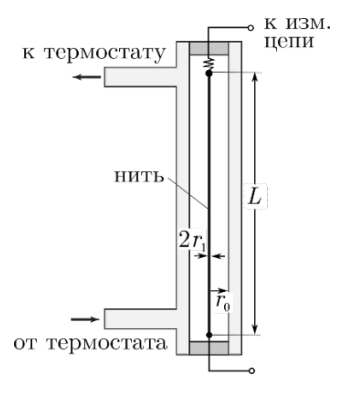
\includegraphics[width=0.9\linewidth]{img/ustanovka.png}
            \caption{Схема экспериментальной установки}
            \label{fig:1}
        \end{figure}
        Углекислый газ подается под давлением через змеевик 5 из баллона 6. Бедный змеевик омывается водой и нагревает газ до температуры воды в термостате.

        Давление газа измеряется манометром М и регулируется вентилем В. Манометр показывает разницу между давлением внутри трубки и атмосферой. Поэтому нормальное показание манометра равно нулю.

        Разность температур газа до и после перегородки измеряется дифференциальной термопарой медь---константан. С помощью вольтметра 7 измеряется разность потенциалов $V$, которая возникает из-за разницы температур. Зависимость $V(t)$ не является линейной, однако в этой работе измеряются малые перепады температур, поэтому этим можно пренебречь. Чувствительность термопары также зависит от температуры, поэтому нам была предоставлена таблица коэффициентов $dV/dt$ для разных температур.
    
    \newpage
    \begin{multicols}{2}
    \section{Обработка результатов измерений}
        В результате измерений были получены данные для 4-х различных температур. Для каждой температуры были измерены разницы потенциалов $V$ (которые впоследствии будут переведены в разность температур $\Delta T$) при различных перепадах давления в промежутке от $p=1.5$ atm до $p=4$ atm. Таблицы с полученными данными приведены в приложении.
        
        Величина показания вольтметра в отсутствие потока газа  (постоянные паразитические эффекты) была пренебрежима мала, поэтому не учитывалась.

        Отложив полученные значения по наклону прямой $\Delta T (\Delta p)$ можно определить значения коэффициента $\mu_{\text{J---T}}$.
    \end{multicols}
    \begin{figure}[H]
        \centering
        \begin{tikzpicture}[scale=1.3]
            \begin{axis}[
                ymajorgrids=true,
                xmajorgrids=true,
                xlabel={$\Delta t, \ s$},
                ylabel={$\gamma$},
                legend pos = north west,
                legend style={nodes={scale=1, transform shape}}, 
                legend image post style={mark=*}
            ]
            \addplot[
                only marks,mark=*,color=black,mark size = 1pt
            ]
            plot [error bars/.cd, y dir = both, x dir = both, y explicit, x explicit]
            table[meta=label, x=t, y=gamma, x error = xe, y error=ye]{
                gamma	t	xe	ye	label
                1.222222222	1	0.15	0.089	a
                1.246575342	0.7	0.15	0.089	a
                1.258741259	0.7	0.15	0.089	a
                1.256756757	0.7	0.15	0.089	a
                1.382352941	0.2	0.15	0.089	a
                1.342465753	0.4	0.15	0.089	a
                1.306666667	0.5	0.15	0.089	a
                1.301369863	0.5	0.15	0.089	a
                1.287671233	0.7	0.15	0.089	a
                1.297297297	0.5	0.15	0.089	a
                1.301369863	0.5	0.15	0.089	a
            };
            \end{axis}
        \end{tikzpicture}




        
    \end{figure}
\end{document}